% Part: sets-functions-relations
% Chapter: relations
% Section: trees

\documentclass[../../../include/open-logic-section]{subfiles}

\begin{document}

\olfileid{sfr}{rel}{tre}
\olsection{树}

树是一种在逻辑学各部分都扮演重要角色的特殊偏序。
有限树出现在逻辑的基础部分：例如，可以将公式理解为其分解后的语法树，
而许多推导系统中的推导也取有限树的形式。
%
无限树则已出现在命题逻辑与一阶逻辑的完备性定理证明中，
并贯穿整个数理逻辑。

树的集合论概念与图论中的树概念密切相关。
下面是一棵（有限）树的图示：

\begin{center}
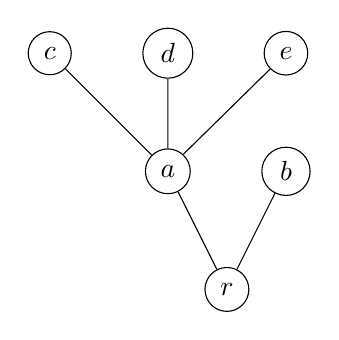
\begin{tikzpicture}[nodes={draw, circle}, -]
\node{$r$} [grow'=up]
    child { node {$a$}
        child { node {$c$} }
        child { node {$d$} }
        child { node {$e$} }
    }
    child { node {$b$} };
\end{tikzpicture}
\end{center}

最底部的节点~$r$ 是\emph{根}。除 $r$ 外的每个节点都恰好有一个紧邻其下的父节点。
如果通过沿边向上追踪能从节点~$x$ 到达节点~$y$，
我们就可以将 $x$ 与 $y$ 之间的关系视为 $x$ 是 $y$ 的\emph{祖先}。

树中的祖先关系是一个严格偏序。这就引出了树的集合论定义。
为给出该定义，我们需要两个概念。
在具有偏序~$\le$ 的集合~$A$ 中，\emph{最小元}是一个元素 $x \in A$，
使得对所有 $y \in A$ 都有~$x \le y$。如果一个集合的每个非空子集都有最小元，
则称该集合被~$\le$ \emph{良序化}。

\begin{defn}[树]
\emph{树}是一个二元组 $T = \tuple{A, \le}$，其中 $A$ 是一个集合，
$\le$ 是 $A$ 上的一个偏序，它具有唯一的最小元 $r \in A$（称为\emph{根}），
且对所有 $x \in A$，集合 $\Setabs{y}{y \le x}$ 都被~$\le$ 良序化。
\end{defn}

\begin{defn}[后继]
设 $T = \tuple{A, \le}$ 是一棵树。
如果 $x,y \in A$，$x < y$，并且不存在 $z \in A$ 使得 $x < z < y$，
那么我们就说 $y$ 是 $x$ 的\emph{后继}。
\end{defn}

$x \in A$ 的后继也称为它的\emph{孩子}。如果 $y$ 是 $x$ 的后继，那么我们称 $x$ 为 $y$ 的\emph{前驱}或\emph{父节点}。

\begin{prop}
如果 $\tuple{A,\le}$ 是一棵树，那么除根节点外，每个 $x \in A$ 至多有一个前驱。
\end{prop}

\begin{proof}
  假设 $y_1 < x$ 且 $y_2 < x$ 且 $y_1 \neq y_2$。那么 $\{y_1,
  y_2\} \subseteq \Setabs{z}{z<x}$。由于 $\Setabs{z}{z<x}$ 被~$\le$ 良序化，其子集 $\{y_1, y_2\}$ 有最小元，
  这个最小元显然必须是 $y_1$ 或~$y_2$。所以要么 $y_1 \le y_2$，要么 $y_2 \le y_1$。我们假设了 $y_1 \neq y_2$，
  所以实际上要么 $y_1 < y_2$，要么 $y_2 < y_1$。由于我们假设了 $y_1 < x$ 且 $y_2 < x$，
  那么进一步有要么 $y_1 < y_2 < x$，要么 $y_2 < y_1 < x$。所以 $y_1$ 和 $y_2$ 不可能同时是 $x$ 的前驱。
\end{proof}

\begin{defn}
若树 $T = \tuple{A, \le}$ 中的 $A$ 是无限集，则称 $T$ 是\emph{无限的}，否则称其为\emph{有限的}。
若 $T$ 中的每个 $x \in A$ 都只有有限多个后继，则称 $T$ 是\emph{有限分支的}。
\end{defn}

\begin{defn}[分支]
给定一棵树 $T = \tuple{A, \le}$，$T$ 的一个\emph{分支}是 $T$ 中的一个极大链，
即一个集合 $B \subseteq A$，使得对任意 $x, y \in B$，要么 $x \le y$，要么 $y \le x$，
并且对任意 $z \in A \setminus B$，存在 $u \in B$ 使得 $z \le u$ 与 $u \le z$ 均不成立。
%
我们用 $[T]$ 表示 $T$ 的所有分支的集合。
\end{defn}

\begin{ex}
有限分支树的一个经典例子是由 $0$ 和~$1$ 的有限序列构成的\emph{无限二叉树}，
有时记作 $\{0,1\}^*$ 或~$\Bin^*$，以扩张关系 $\sqsubseteq$ 为序（例如，$101 \sqsubseteq 101101$）。
由于任何二进制串总可以通过在末尾添加 $0$ 或 $1$ 来扩张，这棵树包含无限多个元素：
每个元素~$s$ 恰好有两个后继，$s0$ 和~$s1$。它的根是空序列 $\emptyseq$。
\end{ex}

\begin{ex}
更一般地，自然数的有限序列集~$\Nat^*$ 连同扩张关系~$\sqsubseteq$ 也是一棵树。
它显然不是有限分支的：每个 $s \in \Nat^*$ 都有无限多个后继~$sn$，即对每个 $n \in \Nat$ 都有一个。
任何在~$\sqsubseteq$ 下封闭的 $A \subseteq \Nat^*$ 都是~$\Nat^*$ 的一棵\emph{子树}。
（也就是说，$A$ 满足如果 $s \in A$ 且 $s' \sqsubseteq s$，那么 $s' \in A$。）
所有有限树都能表示为~$\Nat^*$ 的有限子树。
\end{ex}

\begin{prop}[K\H{o}nig引理]
设 $T = \tuple{A,\le}$ 是一个有限分支的无限树，
则 $T$ 有一条无限分支。
\end{prop}

K\H{o}nig引理的一个特例在可计算性理论中被广泛使用，称为\emph{弱K\H{o}nig引理}，其内容如下：任何 $\{0,1\}^*$ 的无限子树都有一条无限分支。

\end{document}